%%!TEX TS-program = pdflatexmk
%%!TEX encoding = UTF-8 Unicode
\documentclass[11pt]{article}
\usepackage[utf8]{inputenc}

\usepackage[letterpaper,body={6.0in,9.5in},vmarginratio=1:1]{geometry}
\usepackage[small,compact]{titlesec}

\usepackage{fourier}
\usepackage[scaled=0.85]{berasans}
\usepackage[scaled=0.85]{beramono}
\usepackage{microtype}


\usepackage{xcolor}
\usepackage[colorlinks, urlcolor=darkgray, linkcolor=darkgray]{hyperref}

\usepackage{graphicx}

\newcommand{\optkey}{\textsf{Opt}}
\newcommand{\ctlkey}{\textsf{Ctl}}
\newcommand{\cmdkey}{\textsf{Cmd}}
\newcommand{\esckey}{\textsf{Esc}}
\newcommand{\tabkey}{\textsf{Tab}}
\newcommand{\shiftkey}{\textsf{Shift}}

\newcommand{\mnu}[1]{\textsf{#1}}
\newcommand{\cmd}[1]{\textsf{#1}}
\newcommand{\To}{\,\(\to\)\,}

\pagestyle{plain}

\usepackage{microtype}
\usepackage{booktabs}

%\pagestyle{empty}

% set | as a command character within verbatim so you can execute commands there
\usepackage{verbatim}
\makeatletter
\addto@hook\every@verbatim{\catcode`|=0}
\makeatother

% define colored items to be inserted in verbatim environments
\usepackage{xcolor}
\setlength{\fboxsep}{0pt}
\newcommand{\selmark}{\colorbox{green}{\rule[-0.5ex]{0ex}{2.1ex}\texttt{•}}}
\newcommand{\selcom}{\colorbox{green}{\rule[-0.5ex]{0ex}{2.1ex}\texttt{•‹comment›}}}
\newcommand{\selcombwra}{\colorbox{green}{\rule[-0.5ex]{0ex}{2.1ex}\texttt{•‹placement: r,R,l,L,i,I,o,O›}}}
\newcommand{\selcomrule}{\colorbox{green}{\rule[-0.5ex]{0ex}{2.1ex}\texttt{•‹lift›}}}

% define a few items for easy use
\newcommand{\fastex}{Fas\hspace{-.15em}\TeX}
\newcommand{\TS}{\textsf{\TeX Shop}}
\newcommand{\TSVersion}{2.30}
\newcommand{\CCT}{\textsf{CommandCompletion.txt}}

\title{Using Command Completion with \\ \TS}
\author{Herbert Schulz\\\small\href{mailto:herbs2@mac.com}{herbs2@mac.com}}
\date{2011/04/19}


\begin{document}
\maketitle
\thispagestyle{empty}

\section*{Introduction}

As of v1.34 \TS\ offered a Command Completion facility that was reasonably powerful, if under-utilized. Command Completion in \TS\ allows continuations (completions) or substitutions (abbreviations) for a set of characters bounded on the left by a \textsf{Word Boundary Character}\footnote{The \textsf{Word Boundary Characters} are space, tab, linefeed(newline), period, comma, semicolon, colon, \{, \}, (, ) or \textbackslash\ (actually the \textsf{TeX Command Character} which can vary in different implementations). The \{ and \textbackslash\ also become part of the expansion.} and triggered by the Escape (\esckey) key.

With the help of the good folks on the \textsf{Mac OS X TeX} e-mail list\footnote{Subscribe by sending an e-mail to <\url{mailto:MacOSX-TeX-on@email.esm.psu.edu}>.}, a \CCT\ file was created along with associated Applescript macros to take advantage of that facility. The completions and abbreviations supplied often contain bullet characters, `\texttt{•}', called Marks\footnote{Previously called Tabs.}, as placeholders for command arguments or to easily get to the end of an environment. Skipping forward and backward to these Marks was accomplished using macros\footnote{The original \CCT\ file, macros and documentation are still available as \textsf{CommandCompletion.zip} from  <\url{http://public.me.com/herbs2/}>.}; the macros jumped to the Marks and selected, or deleted, them. Most of the abbreviations were inspired by those used in the \textsf{\fastex}\footnote{\textsf{\fastex} was developed by Filip G. Machi, Jerrold E. Marsden and Wendy G. McKay. For more information see the \textsf{\fastex} web page, <\url{http://www.cds.caltech.edu/~fastex/}>.} set used with \textsf{TypeIt4Me}\footnote{\textsf{TypeIt4Me}, by Riccardo Ettore, presently a preference pane, allows abbreviation replacement in most OS~X programs with ``dictionaries'' that can be application dependent. See the \textsf{TypeIt4Me} web page, <\url{http://www.typeit4me.com/}>, for more information.}.

Version 2.30 and later of \TS\ offers a built-in and enhanced version of Command Completion inspired by Hugh Neary and Will Robertson. There is no longer a need for the Applescript macros and the arguments of completions can have short comments.

{\bfseries\TS\ 2.36 introduced the ability to switch the Command Completion trigger key between Tab (\tabkey) and the \esckey\ keys in \mnu{TeXShop}\To\mnu{Preferences}\To\mnu{Source}\To\mnu{Command Completion Triggered By:}. Wherever you see \esckey\ in this document use \tabkey\ if you've set that as the trigger.}

{\bfseries Command Completion in \TS\ 2.38 and later preserves indentation.} Also included is an indented version of the \CCT\ file. It is found in \path{~/Library/TeXShop/CommandCompletion/IndentedCC/} and is activated by copying the file located there into \path{~/Library/TeXShop/CommandCompletion/} thus overwriting the version already there. To get the original version of the \CCT\ file back simply move the \path{~/Library/TeXShop/CommandCompletion/} folder to your Desktop and restart \TS.

\section*{Installation}

Simply place this version of \TS\ into \path{/Applications/TeX/}. If you ever started up an older version of \TS\ (earlier than \TSVersion) also follow the directions in the following sub-section.

\subsection*{\CCT}

A new default version of \CCT\ is embedded within this new version of \TS. It will get installed, along with other files, the first time \TS\ runs \emph{unless} you've used \TS\ before. In that case you need to move the \path{~/Library/TeXShop/CommandCompletion/} (\path{~} is your HOME directory) directory to your Desktop and start the new version of \TS; a replacement folder with the new version of \CCT\ will be created.

If you've already added items to the original file you will be able to merge them into the new file after it's created. You can open the new version of \CCT\ by clicking on the \mnu{Source}\To\mnu{Command Completion}\To\mnu{Edit Command Completion File\dots} menu item. The older file \emph{must} be opened with Unicode (UTF-8) encoding: use the \mnu{File}\To\mnu{Open\dots} (\cmd{\cmdkey-O}) menu command and make sure to select the \textsf{Unicode (UTF-8)} encoding before opening your old version in \TS.

\section*{Some of What's New in \TS}

Most important are four interconnected changes to \TS: an addition to the way \TS\ handles completions from \CCT; a new menu that has commands for searching and selecting Marks within completions; the ability to have comments attached to Marks; a new \CCT\ file that takes some advantage of the previous three changes. The following four sub-sections cover each of these changes in more detail. Some minor menu changes are discussed separately.

\subsection*{Changes to Completion Handling}

Completions (in the \CCT\ file) in previous versions of \TS\ could contain a single \verb|#INS#| command for the positioning of the insertion point within the completion.

This version of \TS\ allows completions to have \emph{two} copies of \verb|#INS#| and the text between them is selected. A single \verb|#INS#| behaves the same as before; there is complete backward compatibility with the previous versions of \TS.

\subsection*{The \mnu{Source}\To\mnu{Command Completion}\To\mnu{Marks} Menu}

The new \mnu{Source}\To\mnu{Command Completion}\To\mnu{Marks} menu contains commands to search for, move to and select Marks and Comments. The commands are shown in Table (\ref{tbl:menu}) on page \pageref{tbl:menu}.
\begin{table}
\centering
\begin{tabular}{llp{6.7cm}}
{\bfseries Menu Item} & {\bfseries Shortcut} & {\bfseries Internal Connection} \\
\cmidrule[0.5pt](lr){1-1} \cmidrule[0.5pt](lr){2-2} \cmidrule[0.5pt](lr){3-3}
\sffamily Next Mark & \ctlkey\,-\,\cmdkey\,-\,\textsf{F} & Jump to and select the next Mark and/or Comment. \\
\sffamily Next Mark (Del) & \ctlkey\,-\,\optkey\,-\,\cmdkey\,-\,\textsf{F} & Jump to and select the next Mark and/or Comment and delete the Mark. This is most useful when you have nested environments to automatically delete a Mark at the end of an inner environment.  \\
\sffamily Previous Mark & \ctlkey\,-\,\cmdkey\,-\,\textsf{G} & Like \textsf{Next Mark} but search backwards. \\
\sffamily Previous Mark (Del) & \ctlkey\,-\,\optkey\,-\,\cmdkey\,-\,\textsf{G} & Like \textsf{Next Mark (Del)} but search backwards. \\
\sffamily Insert Mark & \cmdkey\,-\,\textsf{8} & Places a Mark at the insertion point. Used to mark arguments, etc., when creating new completions in \CCT. \\
\sffamily Insert Comment & \ctlkey\,-\,\cmdkey\,-\,\textsf{8} & Places a Comment Skeleton, ``•‹›'' with the insertion point before the ``›'', at the insertion point. Handy for creating comments in \CCT. \\
\end{tabular}
\caption{Commands in the \mnu{Source}\To\mnu{Command Completion}\To\mnu{Marks} Menu.}
\label{tbl:menu}
\end{table}
The \mnu{(Del)} versions of the search commands only show in the menu when the Option (\optkey) key is pressed and the \texttt{Insert Comment} command only appears when you hold down the Control (\ctlkey) key. The \mnu{Insert Mark} command is added since using \TS's Key Binding (previously called Auto Complete) facility will insert \texttt{\textbackslash bullet} in the document when the keystroke that normally inserts a `•' (\mnu{\optkey-8} with a \textsc{US} keyboard mapping) is pressed. The default version of the \mnu{Marks} menu is shown in Figure (\ref{fig:marks}) on page \pageref{fig:marks}.
\begin{figure}
\centering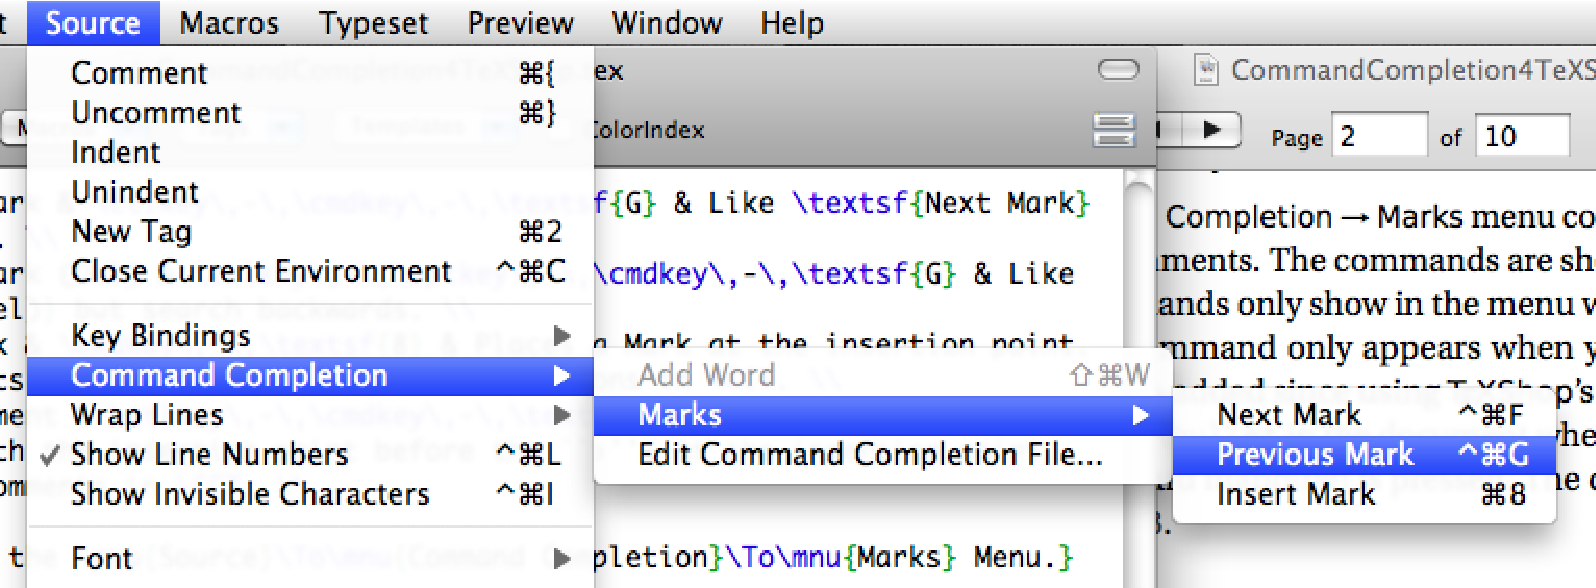
\includegraphics[width=5.5in]{figs/DefaultMarksMenu}
\caption{The Default \mnu{Source}\To\mnu{Command Completion}\To\mnu{Marks} Menu.}
\label{fig:marks}
\end{figure}

\subsection*{Comments}

The changes mentioned in the previous sub-sections allow completions to contain Comments---short ``memory joggers'' that have some information about the contents of a given argument. The comments are contained within arguments and are surrounded by ``•‹'' and ``›\footnote{Note that `\texttt{‹}' and `\texttt{›}' are single ``guillemot'' glyphs, not `<' and `>'.}'' within the arguments; if the first argument contains a comment it should be surrounded by two \verb|#INS#| so it is the initial selection.

\subsection*{The New \CCT\ File}

There are a few changes to the new \CCT\ file that comes with this version of \TS\ when compared to the one supplied with the original add-on version:
\begin{itemize}
\item
there are some minor bug fixes and a few additional environments and commands;
\item
all single \verb|#INS#| commands are replaced by \verb|#INS#•#INS#| so that the initial selection is a selected Mark, \selmark. This is for consistency with the appearance and behavior when using the \texttt{Next/Previous Mark} commands;
\item
there are a few (too few?) examples of comments in commands and environments.
\end{itemize}

\subsection*{Additional Shortcuts in \TS\ 2.36 and Later}

Besides \ctlkey\,-\,\cmdkey\,-\,\texttt{F/G} for \mnu{Next/Previous Mark} \TS\ 2.36 introduced the \optkey/\ctlkey\,-\,\esckey\ as alternates for those menu items. If you wish to turn that feature off execute the command
\begin{verbatim}
defaults write TeXShop CommandCompletionAlternateMarkShortcut NO
\end{verbatim}
in \texttt{Terminal} to turn it off or substitute \texttt{YES} for \texttt{NO} in the command to turn it back on.

\section*{Usage}

\subsection*{Command Completion}

A typical use of command completion is to set up environments. To do this type \verb|\b| and \esckey; this should get you \verb|\begin{|. Then start to type the environment name; e.g., \verb|eq| and \esckey\ will give
\begin{verbatim}
\begin{equation}
|selmark
\end{equation}•
\end{verbatim}
while the next \esckey\ gives \texttt{eqnarray} followed by it's \texttt{*}-variant. After entering your equation text at the cursor run the \mnu{Source}\To\mnu{Completion}\To\mnu{Marks}\To\mnu{Next Mark} command and the cursor will select (and  delete if \mnu{Next Mark (Del)} is used) the next `\texttt{•}' so you can start to type following text.

The macros are also handy for commands that take multiple arguments. For example, to create a new command with an optional argument type \verb|\new| or \verb|\newc| and then \esckey\ three times to get
\begin{verbatim}
\newcommand{|selmark}[•][•]{•}
\end{verbatim}
with the first mark selected. After entering the new command's name use the \texttt{Next Mark} command to jump to the next argument, etc.

\subsection*{Abbreviations}

In addition to command completion there also exist many abbreviations for commands. The principal difference is that the abbreviations are not just the start of a command name. For example typing \texttt{benu} and then \esckey\ \emph{at the beginning of a line}\footnote{Or after any other \texttt{Word Boundary Character}.} will produce the complete enumerated list environment:
\begin{verbatim}
\begin{enumerate}
\item
|selmark
\end{enumerate}•
\end{verbatim}
as you might expect. Abbreviations like this exist for many environments as well as sectioning commands. Alternate command versions with one or more options or \texttt{*}-variants have names that end with `\texttt{o}' (one or more) or `\texttt{s}' respectively: e.g., \texttt{sec} and two presses of \esckey\ or \texttt{secs} and a single \esckey\ at the start of a new line give \verb|\section*{|\selmark\verb|}|. By the way, After typing the text for the first item, typing \texttt{it} and \esckey\ on a new line will generate another \verb|\item| with a selected Mark on the line below it; continued presses of \esckey\ will give \verb|\item[|\selmark\verb|]| with a Mark on the following line, \verb|\textit{|\selmark\verb|}| and finally \verb|\itshape| before returning to the original \texttt{it}.

You must remember to have one of the \textsf{Word Boundary Characters} before use or the substitution won't operate properly. This a not a problem with environments and sectioning commands, since you usually start them on a new line, but can be for other abbreviations. Therefore many abbreviation also have a `\verb|\|' version; e.g., \texttt{\`{}tt} and \esckey\ will not expand properly since the `\texttt{\`{}}' isn't a \textsf{Word Boundary Character} while \texttt{\`{}\textbackslash tt} and \esckey\ will expand to \texttt{\`{}\textbackslash texttt\{\selmark\}} while a second \esckey\ will give the declaration \texttt{\`{}\textbackslash ttfamily}\footnote{Similar abbreviations exist for \texttt{bf}, \texttt{sf}, \texttt{sc}, etc. Math versions have a preceding \texttt{m}; e.g., \texttt{mbf} and \esckey\ will give \texttt{\textbackslash mathbf\{\selmark\}}.}.

Many of the Greek characters and in-line math versions of the Greek characters have abbreviations with the following rules:
\begin{enumerate}
\item
The abbreviations for Greek characters all start with an `\texttt{x}' and a notation for the character: e.g., \verb|xa| or \verb|\xa|\footnote{All of the Greek character abbreviations have \texttt{\textbackslash} versions.} and \esckey\ give \verb|\alpha|. 
\item
The \texttt{var} version of several Greek characters start with `\texttt{xv}' and the notation for the character: e.g., \texttt{xth} gives \verb|\theta| while \verb|xvth| and \esckey\ gives \verb|\vartheta|.
\item
To get capitals for some letters use an `\texttt{xc}': e.g., \verb|xg| gives \verb|\gamma| while \verb|xcg| gives \verb|\Gamma|.
\item
Finally, preceding by a `\texttt{d}' gives the following Greek character as an in-line math equation: e.g., \verb|dxcd| gives \verb|\(\Delta\)|.
\end{enumerate}

Abbreviations will be completed and cycle through matches just like the command completions: e.g., both the abbreviation \texttt{newcoo} (note the `\texttt{oo}' at the end of the abbreviation) and \esckey\ or \texttt{newc} followed by three \esckey\ key presses on a new line give \verb|\newcommand{|\selmark\verb|}[•][•]{•}|, the \verb|\newcommand| with two optional arguments. There are alternate abbreviations for some commands: e.g., \texttt{ncm} gives the same result as \texttt{newc}.

I suggest that you read through the \CCT\ file to see what abbreviations are available; all lines with `\kern-1.7pt\texttt{:=}' are abbreviations. Naturally, you can change them to suit your needs and add and delete others.

\subsection*{Comments}

It is easy to remember the arguments for commands that are used fairly often but to forget those rarely used; these are the perfect candidates for comments. E.g., the order of the arguments for the \verb|\rule| command; type \verb|\rul| and \esckey\ twice to get \verb|\rule[|\selcomrule\verb|]{•‹width›}{•‹height›}|, the version with the optional argument\footnote{This is \texttt{\textbackslash rule[\#INS\#•‹lift›\#INS\#]\{•‹width›\}\{•‹height›\}} in the \CCT\ file.}. Another example is the \texttt{wrapfigure} environment, from the \texttt{wrapfig} package, which has multiple versions with differing numbers and positions of optional arguments. To see the variations with the comments type \texttt{bwr} on an empty line and press \esckey\ to get:
\begin{verbatim}
\begin{wrapfigure}{|selcombwra}{•‹width›}
•
\end{wrapfigure}•
\end{verbatim}
with the versions with optional arguments on succeeding presses of \esckey.

\subsection*{Other Environments}

Environments that aren't built into the \CCT\ file can always be added if you use them a lot but there is an alternative for occasional use. Built into the completion algorithm is a way to complete environments. First press \verb|\b| and \esckey\ to get \verb|\begin{|, enter the environment name and the closing \texttt{\}} and then \esckey\ again; the closing \verb|\end{}| with the corresponding environment name will be generated on a separate line.

\section*{Abbreviations in \CCT}

This section contains a, hopefully, complete list of the abbreviations supplied in the latest \CCT. The list has been broken up into Environments, Commands \& Declarations and Greek Letters. If you supply a certain beginning abbreviation the search will start at the first match to what you supply and succeeding presses of \esckey\ will go down the list until there is no longer a match; e.g. if you type \texttt{be} succeeding presses of \esckey\ will match \texttt{benu}, \texttt{benuo}, \texttt{bequ}, \texttt{bequs}, \texttt{beqn} and \texttt{beqns} before returning to the original \texttt{be}. Adding more letters to the abbreviation may get you to the desired completion with fewer presses of \esckey. In reality some of the Commands \& Declarations are scattered between the Environments in the \CCT\ file so there might be additional items at times. The tables don't include standard completions or the `\verb"\"' versions of the abbreviations.

\textbf{NOTE: The list may be a bit intimidating. There is no need to ``memorize'' all of these abbreviations; learn the minimum number as you need them. In addition variations on a given abbreviation are obtained by successive pressings of \esckey; e.g., see Figure \ref{fig:sec}.}
\begin{figure}\centering
\makebox[\textwidth]{
\fbox{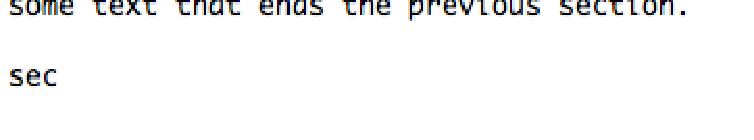
\includegraphics[width=3in]{figs/startsec}}
\hfill\fbox{
\includegraphics[width=3in]{figs/sec}}}
\makebox[\textwidth]{
\fbox{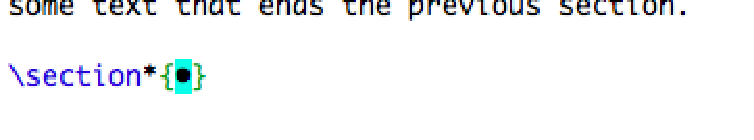
\includegraphics[width=3in]{figs/secs}}
\hfill\fbox{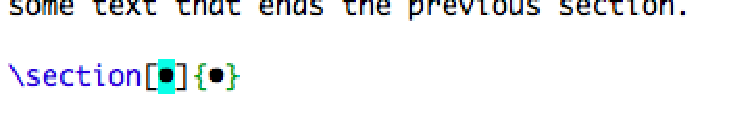
\includegraphics[width=3in]{figs/seco}}}
\caption{Initially entered \texttt{sec} and successive pressings of \esckey\ from initial to last result before returning to the beginning. Corresponds to the sequence \textsf{initial}\To\textsf{sec}\To\textsf{secs}\To\textsf{seco}.}
\label{fig:sec}
\end{figure}

\subsection*{Environment Abbreviations}

Table (\ref{tbl:environments}) on page \pageref{tbl:environments} contains a list of abbreviations for different environments supplied in the \CCT\ file. Multiple vertically adjacent Environments with the same name correspond to variations in number and distribution of possible optional arguments or \texttt{*}-variants. There can also be more than one abbreviation for the same environment.

\subsection*{Commands \& Declarations}

As with Environments there are lots of variations with options and \texttt{*}-variants as well as multiple abbreviations corresponding to the same command. See Table (\ref{tbl:commands}) on page \pageref{tbl:commands}.

\subsection*{Greek Letters}

The Greek Letter abbreviations appear in Table (\ref{tbl:greek}) on page \pageref{tbl:greek}. The in-line equation, i.e., `\texttt{d}', versions of the letters are not shown.

\section*{Making Additions to \CCT}

If you are adding items to the \CCT\ there are a few things you should know about its structure:
\begin{itemize}
\item
Each environment has three entries: a completion that removes the leading \verb|\begin|, i.e., it starts with a leading `\texttt{\{}' and the environment name; two abbreviations that have an abbreviation name without a backslash (\verb|\|) and the same abbreviation with the backslash. Commands may have more forms; the full command as well as abbreviation(s) all with and without a leading \verb|\|.
\item
You should add all the variations with slightly different endings for the abbreviations. I use an `\texttt{o}' at the end of an abbreviation if that variation has an optional argument, `\texttt{oo}' for two optional arguments, `\texttt{s}' for \texttt{s}tarred forms of commands, etc.
\item
The order of similar items in the file \emph{does} make a dramatic difference in the order in which items are found; items placed \emph{later} will be found \emph{earlier} (the file is searched backwards). E.g., the order of items obtained when you press \verb|\b| and then \esckey\ depends purely on the order of matches in the \CCT\ file.
\item
For maximum convenience place a Mark\footnote{Using \mnu{Insert Mark} (\cmdkey-\textsf{8}) from the \mnu{Source}\To\mnu{Completion}\To\mnu{Marks} menu.} within each argument of commands. Surround the very first argument with two \verb|#INS#| commands so it comes out selected. If you want to have a comment in any arguments insert a Comment Skeleton\footnote{Using \mnu{Insert Comment} (\ctlkey-\cmdkey-\textsf{8}) from the \mnu{Source}\To\mnu{Completion}\To\mnu{Marks} menu.} and fill it in.
\end{itemize}
I'd suggest that you take a look in the \CCT\ file for examples.

\section*{Bugs}

The \CCT\ file is usually searched backward from the last item but, on rare occasions, the search direction seems to switch so you don't get matches in the order you expect. You can usually force the search to go back to the ``correct'' direction by pressing \verb+---+ and then \esckey\ three times and then remove the \verb+---+. If that doesn't correct the direction you can use \shiftkey\,-\,\esckey\ to search in the ``other'' direction.

\section*{What's Missing}

Any suggestions are welcome and will be considered for inclusion in later iterations of the Command Completion code.

\vspace{5pt plus 2pt minus 1pt}\noindent
Try it\dots\ I hope you like it.

%\vspace{5pt plus 2pt minus 1pt}\noindent
%Good Luck,\\
%Herb Schulz\\
%(\href{mailto:herbs2@mac.com}{herbs2@mac.com})

\begin{table}
\small
\centering
\begin{tabular}{llll}
\textbf{Abbreviation} & \textbf{Environment} & \textbf{Abbreviation} & \textbf{Environment} \\
\cmidrule[0.5pt](lr){1-1} \cmidrule[0.5pt](lr){2-2} \cmidrule[0.5pt](lr){3-3} \cmidrule[0.5pt](lr){4-4}
barr      & array       & blett   & letter \\
babs      & abstract    & blist   & list \\
bali      & align       & bminp   & minipage \\
balis     & align*      & bminpo  & minipage \\
baliat    & alignat     & bmult   & multline \\
baliats   & alignat*    & bmults  & multline* \\
balied    & aligned     & bpict   & picture \\
baliedat  & alignedat   & bpmat   & pmatrix \\
baliedato & alignedat   & bquot   & quotation \\
bapp      & appendix    & bquo    & quote \\
bbmat     & bmatrix     & bsplit  & split \\
bcase     & cases       & bsubeq  & subequations \\
bcent     & center      & btab    & tabular \\
bcenum    & compactenum & btabs   & tabular* \\
bcenumo   & compactenum & btabx   & tabularx \\
bcitem    & compactitem & btabl   & table \\
bcitemo   & compactitem & btablo  & table \\
bdes      & description & btabls  & table* \\
benu      & enumerate   & btablso & table* \\
benuo     & enumerate   & btbl    & table \\
bequ      & equation    & btblo   & table \\
bequs     & equation*   & btbls   & table* \\
beqn      & eqnarray    & btblso  & table* \\
beqns     & eqnarray*   & btabb   & tabbing \\
bfig      & figure      & bbib    & thebibliography \\
bfigo     & figure      & bindex  & theindex \\
bframe    & frame       & btheo   & theorem \\
bframeo   & frame       & btitpg  & titlepage \\
bflalig   & flalign     & btrivl  & trivlist \\
bflaligs  & flalign*    & bvarw   & varwidth \\
bfll      & flushleft   & bverb   & verbatim \\
bflr      & flushright  & bvers   & verse \\
bgath     & gather      & bwrap   & wrapfigure \\
bgaths    & gather*     & bwrapo  & wrapfigure \\
bgathed   & gathered    & bwrapo2 & wrapfigure \\
bgathedo  & gathered    & bwrapoo & wrapfigure \\
bite      & itemize     &         & \\
biteo     & itemize     &         & \\
\end{tabular}
\caption{Environment abbreviations supplied in \CCT.}
\label{tbl:environments}
\end{table}

\begin{table}
\centering
\small
\makebox[\textwidth]{%
\begin{tabular}{llllll}
\textbf{Abbreviation} & \textbf{Command} & \textbf{Abbreviation} & \textbf{Command} & \textbf{Abbreviation} & \textbf{Command} \\
\cmidrule[0.5pt](lr){1-1} \cmidrule[0.5pt](lr){2-2} \cmidrule[0.5pt](lr){3-3} \cmidrule[0.5pt](lr){4-4} \cmidrule[0.5pt](lr){5-5} \cmidrule[0.5pt](lr){6-6}
\texttt{-{}-}    & textendash        & midr       & midrule        & renewcomo       & renewcommand \\
\texttt{-{}-{}-} & textemdash        & mnorm      & mathnormal     & renewcomoo      & renewcommand \\
\texttt{-{}-{}-} & textemdash w/sp   & msf        & mathsf         & rncm            & renewcommand \\
adlen            & addtolength       & mtt        & mathtt         & rnewc           & renewcommand \\
adcount          & addtocounter      & mit        & mathit         & rncmo           & renewcommand \\
bf               & textbf            & midr       & midrule        & rnewcoo         & renewcommand \\
bfd              & bfseries          & mnorm      & mathnormal     & rncmoo          & renewcommand \\
biblio           & bibliography      & mdd        & mdseries       & rmc             & rmfamily \\
bibstyle         & bibliographystyle & mbox       & mbox           & rbox            & raisebox \\
botr             & bottomrule        & makebox    & makebox        & rboxo           & raisebox \\
bibitem          & bibitem           & mboxo      & makebox        & rboxoo          & raisebox \\
bibitemo         & bibitem           & makebox    & makebox        & sec             & section \\
center           & centering         & mboxoo     & makebox        & secs            & section* \\
chap             & chapter           & mpar       & marginpar      & seco            & section \\
cmidr            & cmidrule          & multic     & multicolumn    & ssec            & subsection \\
cmidro           & cmidrule          & ncol       & space \& space & ssecs           & subsection* \\
em               & emph              & ncm        & newcommand     & sseco           & subsection \\ 
emd              & em                & newc       & newcommand     & sssec           & subsubsection \\
foot             & footnote          & ncmo       & newcommand     & sssecs          & subsubsection* \\
frac             & frac              & newco      & newcommand     & ssseco          & subsubsection \\
fbox             & fbox              & ncmoo      & newcommand     & spar            & subparagraph \\
fboxo            & framebox          & newcoo     & newcommand     & spars           & subparagraph* \\
fboxoo           & framebox          & nct        & newcolumntype  & sparo           & subparagraph \\
geometry         & geometry          & newct      & newcolumntype  & setl            & setlength \\
hw               & headwidth         & newpg      & newpage        & stcount         & stepcounter \\
hw2tw            & headw\(=\)textw   & npg        & newpage        & sf              & textsf \\
href             & href              & nline      & newline        & sfd             & sffamily \\
item             & item              & newlin     & newline        & sc              & textsc \\
ito              & item              & nlen       & newlength      & scd             & scshape \\
incg             & includegraphics   & newlen     & newlength      & sl              & textsl \\
incgo            & includegraphics   & nenv       & newenvironment & sld             & slshape \\
it               & textit            & newenv     & newenvironment & sqrt            & sqrt \\
itd              & itshape           & nenvo      & newenvironment & sqrto           & sqrt \\
latex            & LaTeX             & newenvo    & newenvironment & tt              & texttt \\
latexs           & LaTeX w/sp        & nenvoo     & newenvironment & ttd             & ttfamily \\
latexe           & LaTeXe            & newenvoo   & newenvironment & tw              & textwidth \\
latexes          & LaTeXe w/sp       & pgref      & pageref        & tex             & TeX \\
label            & label             & par        & paragraph      & texs            & TeX w/sp \\
lbl              & label             & pars       & paragraph*     & tilde           & textasciitilde \\
lettrine         & lettrine          & paro       & paragraph      & topr            & toprule \\
lettrineo        & lettrine          & pgs        & pagestyle      & toc             & tableofcontents \\
listf            & listoffigures     & parbox     & parbox         & tableofcontents & tableofcontents \\
listt            & listoftables      & parboxo    & parbox         & tpgs            & thispagestyle \\
rule             & rule              & parboxoo   & parbox         & thispagestyle   & thispagestyle \\
ruleo            & rule              & parboxooo  & parbox         & up              & textup \\
mbf              & mathbf            & pbox       & parbox         & upd             & upshape \\
mrm              & mathrm            & pboxo      & parbox         & url             & url \\
mcal             & mathcal           & pboxoo     & parbox         & usep            & usepackage \\
msf              & mathsf            & pboxooo    & parbox         & usepo           & usepackage \\
mtt              & mathtt            & ref        & ref            & verb            & verb \\ 
mit              & mathit            & renewcom   & renewcommand   & verb2           & verb \\
\end{tabular}
}
\caption{Commands and Declarations in \CCT.}
\label{tbl:commands}
\end{table}

\begin{table}\small\centering
\begin{tabular}{llll}
\textbf{Abbreviation} & \textbf{Command} & \textbf{Abbreviation} & \textbf{Command} \\
\cmidrule[0.5pt](lr){1-1} \cmidrule[0.5pt](lr){2-2} \cmidrule[0.5pt](lr){3-3} \cmidrule[0.5pt](lr){4-4}
xa  & alpha      & xph  & phi \\
xb  & beta       & xcph & Phi \\
xch & chi        & xvph & varphi \\
xd  & delta      & xps  & psi \\
xcd & Delta      & xcps & Psi \\
xe  & epsilon    & xs   & sigma \\
xve & varepsilon & xcs  & Sigma \\
xet & eta        & xvs  & varsigma \\
xg  & gamma      & xz   & zeta \\
xcg & Gamma      & xr   & rho \\
xio & iota       & xvr  & varrho \\
xl  & lambda     & xt   & tau \\
xcl & Lambda     & xth  & theta \\
xm  & mu         & xcth & Theta \\
xn  & nu         & xvth & vartheta \\
xo  & omega      & xu   & upsilon \\
xco & Omega      & xcu  & Upsilon \\
xp  & pi         & xx   & xi \\
xcp & Pi         & xcx  & Xi \\
xvp & varpi      &      & \\
\end{tabular}
\caption{Greek Letters in \CCT. The `\texttt{d}' versions are not shown.}
\label{tbl:greek}
\end{table}

\end{document}
